\documentclass[a4paper,11pt,twocolumn]{article}

\usepackage{aas_macros}

\usepackage[utf8]{inputenc}
\usepackage[T1]{fontenc}
\usepackage{lmodern}
%\usepackage{times}
%\usepackage[margin=2cm]{geometry}
\usepackage[a4paper]{geometry}
\usepackage{amsmath}
\usepackage{mathtools}
\usepackage{graphicx}
\usepackage{multirow}
\usepackage{multicol}
\usepackage{blindtext}
\usepackage{hyperref}
\usepackage{float}

\usepackage{pgfplotstable}
\usepackage{booktabs}
% \pgfplotsset{compat=1.18}

\usepackage[authoryear]{natbib}

\graphicspath{ {./images/} }

\usepackage[czech]{babel}
\usepackage{graphicx}
\usepackage{amsmath}
\usepackage{xspace}
\usepackage{url}
\usepackage{siunitx}
\usepackage{indentfirst}
\usepackage{subcaption}
\usepackage{caption}
\usepackage{tabularx}
\usepackage{rotating}
\usepackage{tikz}
\usepackage[labelformat=parens,labelsep=quad,skip=3pt]{caption}

\usepackage{color}
\usepackage{listings}

\definecolor{codegreen}{rgb}{0,0.6,0}
\definecolor{codegray}{rgb}{0.5,0.5,0.5}
\definecolor{codepurple}{rgb}{0.58,0,0.82}
\definecolor{backcolour}{rgb}{0.95,0.95,0.92}

\lstdefinestyle{mystyle}{
    backgroundcolor=\color{backcolour},
    commentstyle=\color{codegreen},
    keywordstyle=\color{magenta},
    numberstyle=\tiny\color{codegray},
    stringstyle=\color{codepurple},
    basicstyle=\ttfamily\footnotesize\centering,
    breaklines=true,
    captionpos=b,
    numbers=left,
    numbersep=5pt,
    showspaces=false,
    showstringspaces=false,
    showtabs=false,
    tabsize=2
}

\lstset{style=mystyle}

%\widowpenalty 10000 \clubpenalty 10000 \displaywidowpenalty 10000
\setcounter{topnumber}{3}
\setcounter{bottomnumber}{3}
\setcounter{totalnumber}{6}
\renewcommand\topfraction{0.9}
\renewcommand\bottomfraction{0.9}
\renewcommand\textfraction{0.1}
\intextsep=8mm \textfloatsep=8mm

\renewcommand{\thesection}{\arabic{section}.}
\renewcommand{\thesubsection}{\thesection\arabic{subsection}.}
\makeatletter \def\@seccntformat#1{\csname the#1\endcsname\hspace{1ex}} \makeatother


\begin{document}
    \twocolumn[
    \noindent\hrulefill
    \begin{center}
        \bigskip
        \huge Precese perihélia Merkuru
        \vspace{0.2cm}
        \par \large F5330 Základní numerické metody
        \par \large Artem Gorodilov
        \vspace{0.2cm}
        \par \large 8. ~února 2025
        \bigskip
    \end{center}
    \noindent\hrulefill
    \bigskip
    ]

    \vskip10pt

    \section{Abstrakt}
        V této práci jsem provedl modelování precese dráhy Merkuru pomocí druhého Newtonova zákona s korekcí Obecné Teorie Relativity (OTR). Analyzoval jsem účinnost různých parametrů modelu. Zejména jsem našel optimální hodnotu koeficientu $\beta = 1.1 \times 10^5$ a optimální parametry meze integraci $N_{\text{T}} = 150$ a integračního kroku $N_{\text{dt}} = 150$, při kterých se vypočtená hodnota precese bude minimálně lišit od teoretické a chyba hodnoty bude minimální $\varphi = 43.1(3) ~[\text{arcsec/století}]$, se liší o $0.2(8)\%$ od teoretické hodnoty. 
        
        Výpočty byly provedeny pomocí skriptu v Pythonu (viz. \citet{github}).

    \section{Úvod}
        Jedním z nejvýznamnějších experimentálních potvrzení OTR byla přesná předpověď nadbytečné precesní změny perihelia Merkurovy dráhy, která činí přibližně $\varphi_{\text{teor}} = 43.03(3) ~[\text{arcsec/století}]$ \citet{clemence1947}. Tento jev byl dlouhou dobu neobjasněným problémem klasické nebeské mechaniky.

        Podle Newtonovy gravitační teorie by se oběžné dráhy planet měly chovat jako uzavřené elipsy s ohniskem v místě Slunce. Nicméně vzájemné gravitační působení planet způsobuje malé poruchy, které vedou k postupnému otáčení hlavní osy elipsy v rovině dráhy - tento jev se označuje jako precesní pohyb perihelia. U Merkuru je celková pozorovaná hodnota precesního posunu $9.55 ~[\text{arcsec/století}]$, z čehož $8.85 ~[\text{arcsec/století}]$ úhlových minut lze vysvětlit gravitačními interakcemi s ostatními planetami. Zbývající $43.1 ~[\text{arcsec/století}]$ úhlových vteřin za století však zůstávalo nevysvětleno. OTR tento problém vyřešila zavedením relativistické opravy Newtonova gravitačního zákona.    
    
    \section{Model}
        Původní Newtonův pohybový zákon pro gravitační soustavu zní:

        \begin{equation*}
            \vec{F} = m \ddot{\vec{r}} 
        \end{equation*}

        kde $\vec{F}$ je síla působící na těleso, $m$ je hmotnost tělesa, $\vec{r}$ je poloha tělesa a $\ddot{\vec{r}}$ je zrychlení tělesa. Tehdy zrychlení tělesa obíhajícího kolem Slunce lze vyjádřit jako:

        \begin{equation*}
            \ddot{\vec{r}} = -\frac{G M_{\odot}}{r^2} \frac{\vec{r}}{r}
        \end{equation*}

        kde $G$ je gravitační konstanta, $M_{\odot}$ je hmotnost Slunce a $r$ je vzdálenost tělesa od Slunce. To popisuje dokonalou eliptickou dráhu při keplerovském pohybu. Pokud však uvažujeme další efekty, musíme tuto rovnici upravit tak, aby zahrnovala další členy, které aproximují efekty OTR:

        \begin{equation}
            \ddot{\vec{r}} = -\frac{G M_{\odot}}{r^2} \left(1 + \alpha \frac{2 G M_{\odot}}{r c^2} + \beta \frac{L^2}{m_{\text{p}}^2 r^2 c^2}\right) \frac{\vec{r}}{r}
            \label{eq:motion_corr}
        \end{equation}

        kde $\alpha$ a $\beta$ jsou koeficienty, $L$ je moment hybnosti tělesa, $m_{\text{p}}$ je hmotnost planery a $c$ je rychlost světla. 

        Člen

        \begin{equation*}
            \alpha \frac{2 G M_{\odot}}{r c^2}
        \end{equation*}

        je tzv. Schwarzschildova korekce (relativistická gravitační korekce). Tento člen vyplývá z OTR. Koriguje Newtonovu gravitaci na malých vzdálenostech zohledněním zakřivení časoprostoru. Tato korekce zvyšuje sílu gravitace v blízkosti Slunce, čímž modifikuje oběžnou dráhu. Parametr $\alpha$ řídí sílu této korekce. To způsobuje precesi perihelia Merkuru v čase. Místo toho, aby dráha sledovala dokonalou elipsu, pomalu rotuje v důsledku zakřivení časoprostoru.

        Člen

        \begin{equation*}
            \beta \frac{L^2}{m_{\text{p}}^2 r^2 c^2}
        \end{equation*}

        je tzv. Frame-dragging korekce (v závislosti na úhlovém momentu hybnosti). Tento člen závisí na úhlovém momentu hybnosti Merkuru L. Zohledňuje, jak pohyb zakřiveným časoprostorem ovlivňuje dráhu. Někdy je spojován s frame-dragging efekty v silných gravitačních polích \cite{pfister2007}. Moment hybnosty $L^2$ Merkuru lze vypočítat takto:
        
        \begin{equation}
            L^2 = |\vec{r} \times \dot{\vec{r}}|^2 
            \label{eq:angular_momentum}
        \end{equation}

        Tento člen modifikuje pohyb v důsledku skutečnosti, že energie a úhlový moment hybnosti se v relativistické soustavě striktně nezachovávají. Přidává další korekci, která mírně mění precesi perihelia. Její velikost se řídí parametrem $\beta$.

        Koeficienty $\alpha$ a $\beta$ pro Merkur jsou dány OTR \footnote{Všechny parametry Merkuru byly převzaty z:: \url{https://nssdc.gsfc.nasa.gov/planetary/factsheet/mercuryfact.html}}: 
        
        \begin{equation}
            \alpha = 0, \quad \beta = 3
            \label{eq:alpha_beta}
        \end{equation}

    \section{Pipeline}
        \subsection{Počáteční podmínky}
            K vyřešení problému jsem použil metodu intergování pohybu Merkuru po jeho oběžné dráze. Samozřejmě musíme někde začít. Tímto začátkem je poloha Merkuru v periheliu, daná hodnotou $r_{\text{per}}$, která byla vypočtena jako:

            \begin{equation}
                r_{\text{per}} = a(1 - e)
                \label{eq:r_per}
            \end{equation}

            kde $a$ je velká poloosa dráhy a $e$ je excentricita dráhy. Pro Merkur je $a = 57.909 \times 10^9 ~\text{m}$ a $e = 0.2056$.

            K popisu pohybu je zapotřebí tečnou rychlost $\dot{r}_{\text{per}}$ a dostředivé zrychlení $\ddot{r}_{\text{per}}$ v periheliu. Tyto hodnoty byly vypočteny jako:

            \begin{equation}
                \dot{r}_{\text{per}} = \sqrt{\frac{G M_{\odot}}{a} \frac{1 + e}{1 - e}}
                \label{eq:rdot_per}
            \end{equation}

            a

            \begin{equation}
                \ddot{r}_{\text{per}} = \frac{G M_{\odot}}{r_{\text{per}}^2}
                \label{eq:rddot_per}
            \end{equation}

            Získané hodnoty se rovnají: 

            \begin{equation*}
                \begin{aligned}
                    r_{\text{per}} &= 4.6 \times 10^{10} ~\text{m}, \\
                    \dot{r}_{\text{per}} &= 5.9 \times 10^4 ~\text{m/s}, \\
                    \ddot{r}_{\text{per}} &= 0.0627 ~\text{m/s}^2
                \end{aligned}
            \end{equation*}

            $r_{\text{per}}$ a $\dot{r}_{\text{per}}$ jsem spojil do vektorů: 

\begin{lstlisting}[language=Python, caption={Počáteční podmínky}]
# Initial conditions
r0 = np.array([perihelion_distance, 0, 0])  # Mercury starts at perihelion
v0 = np.array([0, v_perihelion, 0])  # tangential velocity at perihelion
\end{lstlisting}

            kde \texttt{perihelion\_distance} je hodnota $r_{\text{per}}$ a \texttt{v\_perihelion} je hodnota $\dot{r}_{\text{per}}$.

            Simulace bude vyžadovat také znalost periody oběžné dráhy Merkuru. Tato hodnota bude použita k určení doby integrace. Pro tento účel bude hodnota periody (jeden celý oběh) vynásobena požadovaným počtem oběhů $N_{\text{T}}$. Oběžná perioda Merkuru je rovna:

            \begin{equation}
                T = 87.969 ~\text{d}
                \label{eq:mer_period}
            \end{equation}  

            Integrační krok $dt$ lze dobře aproximovat pomocí vzorce:

            \begin{equation}
                dt = \frac{2 \dot{r}_{\text{per}}}{\ddot{r}_{\text{per}}} \frac{1}{N_{\text{dt}}}
                \label{eq:dt}
            \end{equation}

            kde pomocí $N_{\text{dt}}$ lze získat požadovaný počet kroků integrace a tím zvýšit přesnost výpočtu.

            \begin{figure}
                \centering
                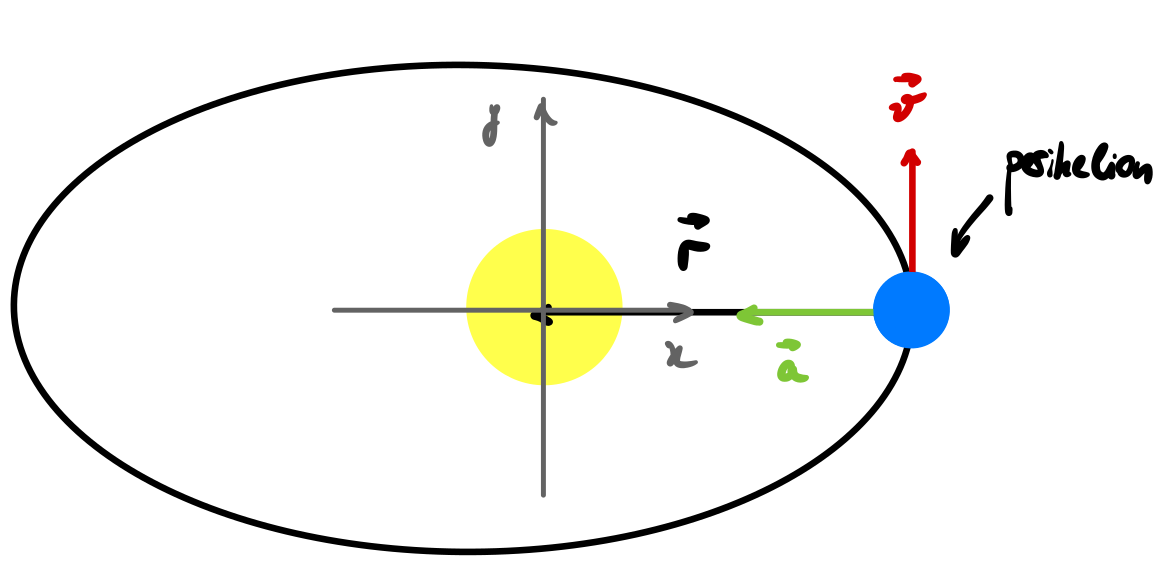
\includegraphics[width=0.5\textwidth]{ms_scheme.png}
                \caption{Systema Merkur-Slunce a základní parametry.}
                \label{fig:ms_scheme}
            \end{figure}

        \subsection{Simulace}
            Integrace se provádí pomocí funkce \texttt{simulate\_orbit()}, která jako vstupní parametry přijímá \texttt{alpha}, \texttt{beta}, \texttt{$\text{N}_\text{T}$} a \texttt{$\text{N}_\text{dt}$}. Tato funkce vrací vektor polohy Merkuru v průběhu času $\vec{r}$. 
            
            
\begin{lstlisting}[language=Python, caption={Simulace oběhu}]      
def simulate_orbit(alpha, beta, N_T, N_dt):
    T, dt, steps = time_parameters(N_T, N_dt)
    
    r = np.zeros((steps, 3))
    v = np.zeros((steps, 3))
    
    r[0] = r0
    v[0] = v0
    
    for i in range(steps - 1):
        a = acceleration(r[i], v[i], alpha, beta)

        v[i+1] = v[i] + a * dt * 86400  # days to seconds
        r[i+1] = r[i] + v[i+1] * dt * 86400

    return r    
\end{lstlisting}
            
            Funkce vypočítá celkovou dobu integrace \texttt{T} a integrační krok \texttt{dt} pomocí funkce \texttt{time\_parameters()}, která jako vstup přijme \texttt{$\text{N}_\text{T}$} a \texttt{$\text{N}_\text{dt}$} a vrátí \texttt{T}, \texttt{dt} a počet integračních kroků \texttt{steps}. 

\begin{lstlisting}[language=Python, caption={Parametry integrace}]
def time_parameters(N_T, N_dt):
    T = N_T * T_mercury # iteractions in days
    dt = (2 * v_perihelion / a_perihelion) / 86400 / N_dt # days

    steps = int(T / dt)
    
    return T, dt, steps
\end{lstlisting}

            Funkce \texttt{simulate\_orbit()} vytvoří pole \texttt{r} a \texttt{v} pro uložení vektorových dat polohy a rychlosti. Jako počáteční vektory bereme jejich hodnoty v perehelu vypočtené dříve. Funkce pak pomocí cyklu \texttt{acceleration()} vypočítá zrychlení pro každou polohu planety při jejím oběhu. 

            Tato funkce je nejdůležitější, protože je zodpovědná za precesi Merkurova perehelia. Funkce přijímá jako vstup vektor polohy planety \texttt{r}, rychlost \texttt{v} a koeficienty \texttt{alpha} a \texttt{beta}. Funkce provede vektorové transformace pro výpočet momentu hybnosti \texttt{L} a vypočítá jej podle vzorce (\refeq{eq:angular_momentum}). Dále funkce vypočítá korekční člen v závorkách v rovnici (\refeq{eq:motion_corr}). Poté funkce vypočítá vektor zrychlení \texttt{a} podle vzorce (\refeq{eq:motion_corr}) a vrátí jeho hodnotu.

\begin{lstlisting}[language=Python, caption={Výpočet zrychlení}]
def acceleration(r, v, alpha, beta):
    r_mag = np.linalg.norm(r)  # calculating the magnitude of the position vector
    r_unit = r / r_mag  # unit vector in the direction of r
    
    # Calculating angular momentum squared term: (r vec * r vec dot)^2 / c^2
    L_squared = np.linalg.norm(np.cross(r, v))**2 / c**2
    
    # Calculating the relativistic correction factors
    correction_term = 1 + (alpha * 2 * G * M_sun) / (r_mag * c**2) + beta * L_squared / r_mag**2
    
    # Calculating the acceleration vector
    a = -G * M_sun / r_mag**2 * correction_term * r_unit
    
    return a 
\end{lstlisting}

        \subsection{Vypočet precese}
            Získáním vektorů polohy planety v čase můžeme ověřit, že dráha Merkuru je skutečně precesní. To lze provést vizuální analýzou dráhy, kterou planeta urazila během doby integrace. Výsledek je znázorněn na obrázku (\ref{fig:orbit}).

            \begin{figure}
                \centering
                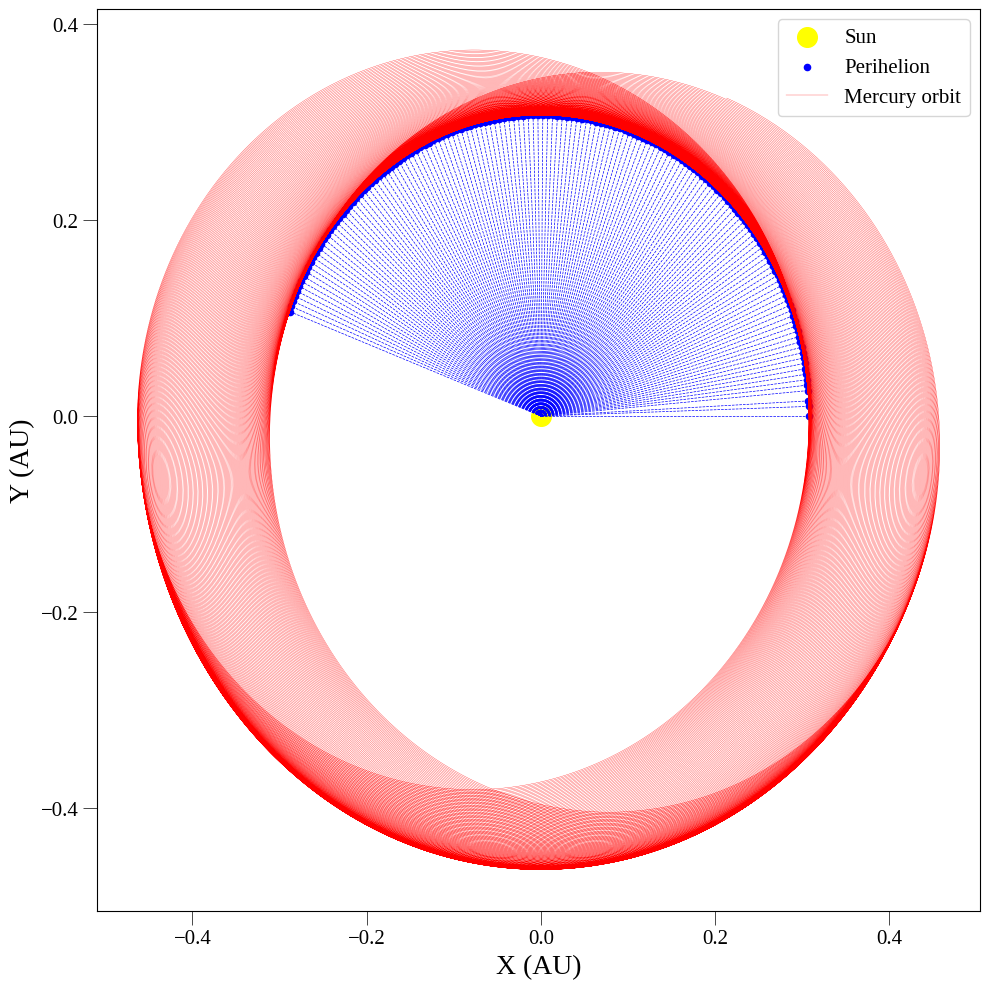
\includegraphics[width=0.5\textwidth]{orbit_0_110000.0_150_150.png}
                \caption{Oběžná dráha Merkuru s precesí perihélia. Parametry: $\alpha = 0$, $\beta = 1.1 \times 10^5$, $N_{\text{T}} = 150$, $N_{\text{dt}} = 150$.}
                \label{fig:orbit}
            \end{figure}

            Abychom mohli vypočítat precesi perihelia Merkuru, musíme zjistit všechny polohy perihelia Merkuru a poté zjistit úhlový posun perihelia mezi dvěma po sobě jdoucími polohami. K tomu jsem použil funkci \texttt{find\_perihelion\_positions()}, která přijímá vektor poloh Merkuru \texttt{r} a vrací pole poloh Merkuru v periheliu a jejich chyby. Funkce funguje následovně: cyklem prochází všechny polohy planety a hledá tři polohy A, B a C, které následují (viz obrázek \ref{fig:per_scheme}). Bod $r_\text{B}$ bude perehelem, pokud $r_\text{B} < r_\text{A}$ a $r_\text{B} < r_\text{C}$. Pokud je tato podmínka splněna, je poloha $r_\text{B}$ přidána do pole poloh perihelia. Chyba polohy perihelia se aproximuje jako střední hodnota rozdílu mezi $r_\text{A}$ a $r_\text{C}$.

\begin{lstlisting}[language=Python, caption={Výpočet poloh perihelia}]
def find_perihelion_positions(r):
    r_magnitude = np.linalg.norm(r, axis=1)
    perihelion_positions = [r[0]]  # starting with the initial perihelion
    uncertainties = []
    
    for i in range(1, len(r_magnitude) - 1):
        if r_magnitude[i] < r_magnitude[i - 1] and r_magnitude[i] < r_magnitude[i + 1]:
            perihelion_positions.append(r[i])
            uncertainty = abs(r_magnitude[i+1] - r_magnitude[i-1]) / 2  # approximation of positional uncertainty
            uncertainties.append(uncertainty)

    first_uncertainty = np.mean(uncertainties)
    uncertainties.insert(0, first_uncertainty)
    
    return np.array(perihelion_positions), np.array(uncertainties)
\end{lstlisting}

            \begin{figure}
                \centering
                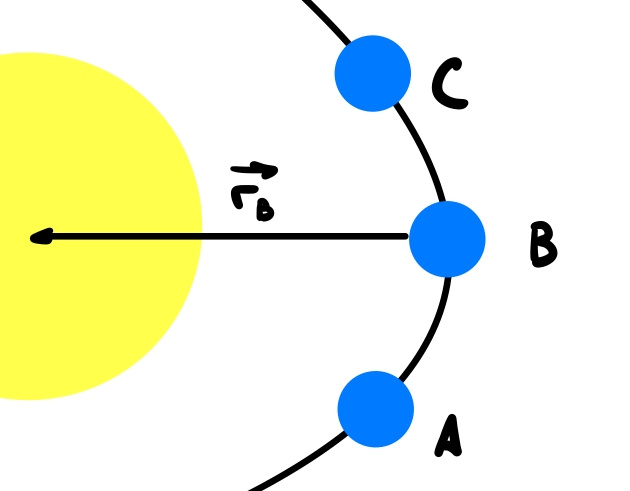
\includegraphics[width=0.5\textwidth]{per_pos_scheme.png}
                \caption{Schéma hledání polohy perihelia.}
                \label{fig:per_scheme}
            \end{figure}

            Samotná precese je definována jako úhlový posun perihelia mezi dvěma po sobě následujícími polohami $\vec{r_1}$ a $\vec{r_2}$. Úhel mezi těmito dvěma vektory je definován jako: 

            \begin{equation}
                \cos{\theta} = \frac{\vec{r_1} \cdot \vec{r_2}}{|\vec{r_1}||\vec{r_2}|}
                \label{eq:cos}
            \end{equation}

            Dot Product vektorů $\vec{r_1}$ a $\vec{r_2}$ je definován jako:

            \begin{equation}
                \vec{r_1} \cdot \vec{r_2} = x_1 x_2 + y_1 y_2
                \label{eq:dot}
            \end{equation}

            Velikosti vektorů $\vec{r_1}$ a $\vec{r_2}$ jsou definovány jako:

            \begin{equation}
                    |\vec{r_1}| = \sqrt{x_1^2 + y_1^2}, ~|\vec{r_2}| = \sqrt{x_2^2 + y_2^2}
                \label{eq:mag}
            \end{equation}

            Dosazením (\refeq{eq:dot}) a (\refeq{eq:mag}) do (\refeq{eq:cos}) a řešením pro $\theta$ získáme úhlové posunutí mezi oběma vektory:

            \begin{equation}
                \theta = \arccos{\left(\frac{x_1 x_2 + y_1 y_2}{\sqrt{x_1^2 + y_1^2} \sqrt{x_2^2 + y_2^2}}\right)}
                \label{eq:theta}
            \end{equation}

            K výpočtu se používá funkce \texttt{calculating\_perihelion\_angles()}, která bere vektory polohy planety a jejich chyby a vrací průměrný úhlový posun perihelia a jeho chybu. 

\begin{lstlisting}[language=Python, caption={Výpočet úhlového posunu perihelia}]
def calculating_perihelion_angles(positions , uncertainties):
    angles_val = []
    angles_err = []
    for i in range(1, len(positions)):
        position_x_1 = ufloat(positions[i-1][0], uncertainties[i-1])
        position_y_1 = ufloat(positions[i-1][1], uncertainties[i-1])

        position_x_2 = ufloat(positions[i][0], uncertainties[i])
        position_y_2 = ufloat(positions[i][1], uncertainties[i])

        phi = um.acos((position_x_1 * position_x_2 + position_y_1 * position_y_2) / (um.sqrt(position_x_1**2 + position_y_1**2) * um.sqrt(position_x_2**2 + position_y_2**2)))
        angles_val.append(um.degrees(phi).nominal_value)
        angles_err.append(um.degrees(phi).std_dev)

    average_precession = ufloat(np.mean(angles_val), uncert(angles_val, np.mean(angles_err)))

    return average_precession
\end{lstlisting}

            Pro určení úhlu posunu perehelia za století v akresekundách je třeba určit poměr pozemského roku k merkurovskému roku:

            \begin{equation*}
                T_{\text{rel}} = \frac{T_{\text{Earth}}}{T_{\text{Mercury}}} = \frac{365.256}{87.969} = 4.152
            \end{equation*}

            Pak úhel posunu perehelia za století v akresekundách je roven:

            \begin{equation}
                \varphi = \frac{\varphi_{\text{deg}}}{T_{\text{rel}}} \times 3600 \times 100 \frac{(k_{\beta}, k_{\alpha})}{(\alpha, \beta)}
                \label{eq:phi}
            \end{equation}

            Poslední násobitel v rovnici (\refeq{eq:phi}) je nutný pro škálování výsledku na koeficienty $\alpha$ a $\beta$. Z (\refeq{eq:alpha_beta}) vyplývá, že $k_{\alpha} = 0$ a $k_{\beta} = 3$. Hodnoty $\alpha$ a $\beta$ budou vysvětleny a vypočteny v následující části. Rovnice (\refeq{eq:phi}) bude vypadat takto:

            \begin{equation}
                \varphi = \frac{\varphi_{\text{deg}}}{T_{\text{rel}}} \times 3600 \times 100 \frac{3}{\beta}
                \label{eq:phi_final}
            \end{equation}

        K výpočtu veličin a jejich nejistot byla použita knihovna Uncertinties pro Python. Chyby byly rozšířeny o Studentův koeficient (2-Tail Confidence Level) s ohledem na stupně volnosti pro každou hodnotu, pro interval spolehlivosti 68.27\%.

    \section{Analýza výsledků}
        \subsection{Optimální hodnoty koeficientů $\alpha$ a $\beta$}

            Pro získání odpovídající hodnoty úhlu posunu perehelia je třeba zvolit potřebné hodnoty koeficientů $\alpha$ a $\beta$. Z (\refeq{eq:alpha_beta}) vidíme, že hodnoty $\alpha$ a $\beta$ pro Merkur jsou resp. 0 a 3. Pokud však provedeme simulace s těmito hodnotami, posun perehelia nepozorujeme. To je dobře vidět na obrázku (\ref{fig:phi_alpha}), který ukazuje lineární závislost úhlu posunu perehelia $\varphi$ na hodnotě koeficientu $\beta$ při pevné hodnotě $\alpha = 0$. Jak je vidět, posun se stává znatelným při hodnotách $\beta \approx \times 10^5$.
            
            \begin{figure}
                \centering
                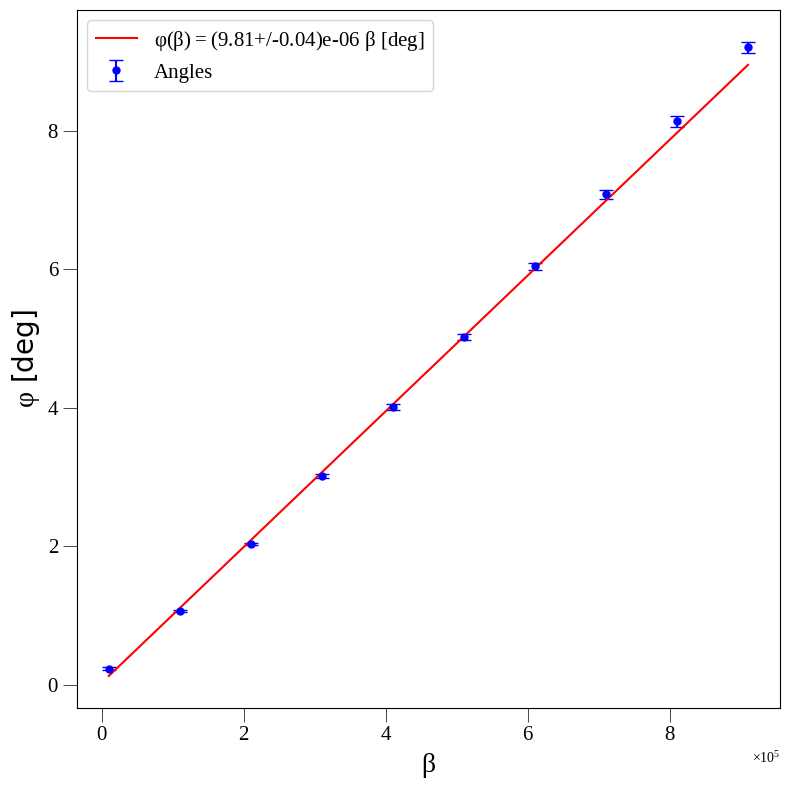
\includegraphics[width=0.5\textwidth]{phi_alpha.png}
                \caption{Závislost úhlu posunu perehelia na hodnotě koeficientu $\beta$ při $\alpha = 0$.}
                \label{fig:phi_alpha}
            \end{figure}

            Totéž se stane, pokud stanovíme $\beta = 0$ a změníme $\alpha$. Jak je patrné z obrázku (\ref{fig:phi_beta}), úhlový posun perihelia je patrný při hodnotách $\alpha \approx \times 10^5$.

            \begin{figure}
                \centering
                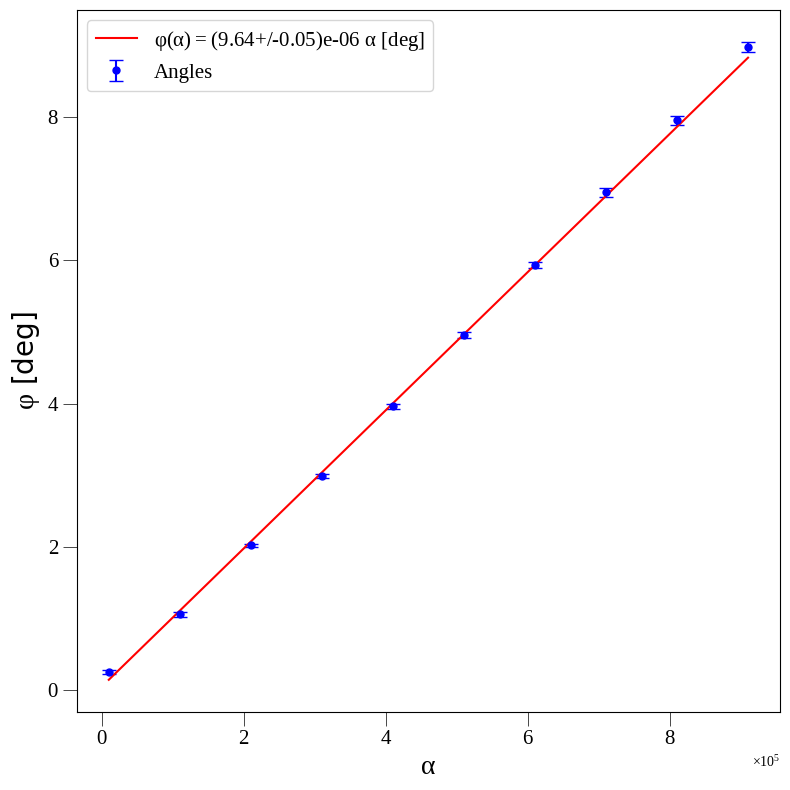
\includegraphics[width=0.5\textwidth]{phi_beta.png}
                \caption{Závislost úhlu posunu perehelia na hodnotě koeficientu $\alpha$ při $\beta = 0$.}
                \label{fig:phi_beta}
            \end{figure}

            Vyvstává otázka, jak zvolit optimální hodnoty koeficientů $\alpha$ a $\beta$, aby se průměrná hodnota úhlu posunutí perehelia co nejméně lišila od teoretické hodnoty? Za tímto účelem jsem provedl sérii simulací s různými hodnotami $\beta$ při pevných hodnotách $\alpha = 0$ a $\alpha$ při pevných hodnotách $\beta = 0$. Simulace byly provedeny pro různé hodnoty integračních kroků $dt/N_{\text{dt}}$. Integrační interval byl ve všech situacích stejný $TN_{\text{T}} = 90T$.  
            
            Výsledky jsou uvedeny na obrázcích (\ref{fig:phi_alpha_diff}) a (\ref{fig:phi_beta_diff}). Výpočty byly provedeny pomocí funkce \texttt{getting\_angle\_data()}, která vypočítá hodnoty úhlů perehelia pro různé hodnoty $\alpha$ a $\beta$, načež funkce \texttt{plotting\_difference()} vypočítá relativní odchylku od teoretické hodnoty a vykreslí závislost této odchylky na $\alpha$ a $\beta$. 

            \begin{figure}
                \centering
                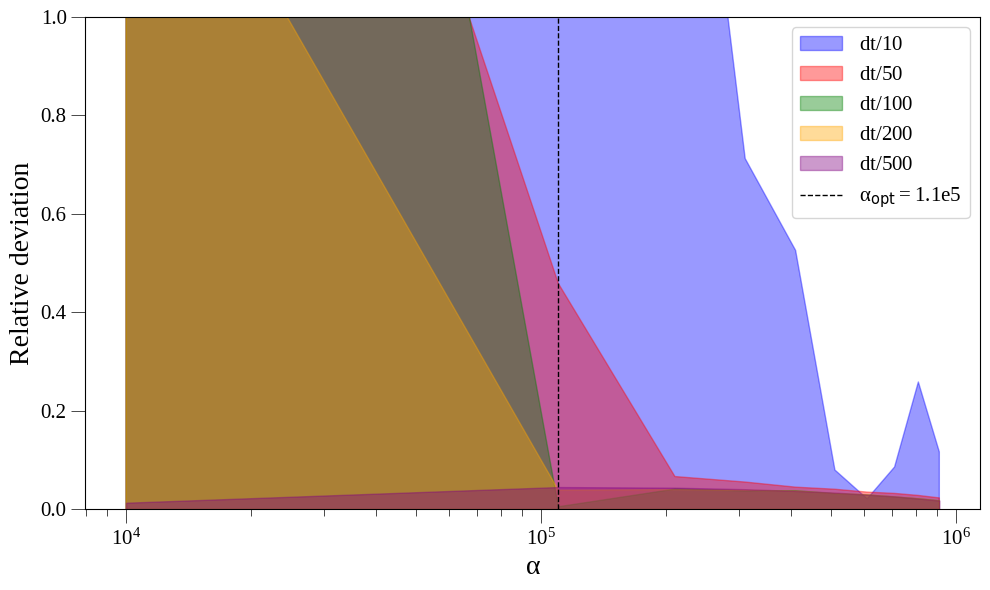
\includegraphics[width=0.5\textwidth]{phi_alpha_diff.png}
                \caption{Závislost odchylky úhlu posunu perehelia od teoretické hodnoty na hodnotě koeficientu $\beta$ při $\alpha = 0$.}
                \label{fig:phi_alpha_diff}
            \end{figure}

            \begin{figure}
                \centering
                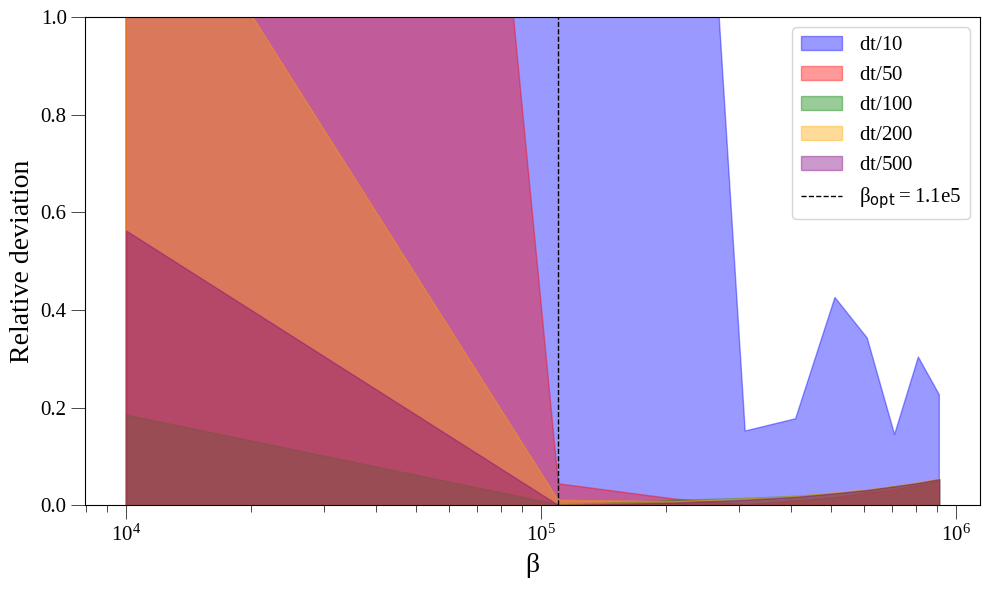
\includegraphics[width=0.5\textwidth]{phi_beta_diff.png}
                \caption{Závislost odchylky úhlu posunu perehelia od teoretické hodnoty na hodnotě koeficientu $\alpha$ při $\beta = 0$.}
                \label{fig:phi_beta_diff}
            \end{figure}

            Z obrázků je patrné, že velikost relativní chyby závisí na velikosti integračního kroku. Například při $dt/10$ je relativní chyba vysoká v celém rozsahu hodnot $\alpha$ a $\beta$. Se zmenšováním integračního kroku je zřejmé, že nejmenší relativní chyba je dosažena při hodnotách $\beta \approx 1.1 \times 10^5$  $\alpha \approx 1.1 \times 10^5$. 

            Právě tato hodnota by měla být použita při simulaci a později bude použita jako hodnota $\beta$ ve vzorci (\refeq{eq:phi_final}) pro výpočet úhlu posunu perehelia za století.

        \subsection{Optimální hodnoty integračních kroků a intervalu integrace} 
        \label{sec:optimal}
            Je velmi důležité správně definovat integrační krok a integrační interval. Oba tyto parametry ovlivňují přesnost a dobu výpočtu. Minimalizace těchto parametrů vyžaduje analýzu funkce dvou proměnných $\sigma(\text{N}_{\text{T}}, \text{N}_{\text{dt}})$, kde $\sigma$ je relativní odchylka precesního úhlu od teoretické hodnoty, $\sigma_{\text{err}}$ je chyba odchylky a $t_{\text{compute}}(\text{N}_{\text{T}}, \text{N}_{\text{dt}})$ je doba výpočtu.
            
            Abych zjistil optimální hodnoty těchto parametrů, provedl jsem test efektivity pomocí funkce \texttt{efficiency\_test()}. Tato funkce přijímá jako vstup hodnoty $\alpha$ a $\beta$ a pole hodnot $\text{N}_{\text{T}}$ a $\text{N}_{\text{dt}}$ v následujících rozmezích: $10 < \text{N}_{\text{T}} < 200$ a $10 < \text{N}_{\text{T}} < 500$ v přírůstcích po 10 bodech. Funkce vrací pole hodnot $\sigma$, $\sigma_{\text{err}}$ a $t_{\text{compute}}$ pro každou kombinaci $\text{N}_{\text{T}}$ a $\text{N}_{\text{dt}}$. Vysledky jsou zobrazeny na obrázcích (\ref{fig:3d_deviation}) a (\ref{fig:3d_time}).

            \begin{figure}
                \centering
                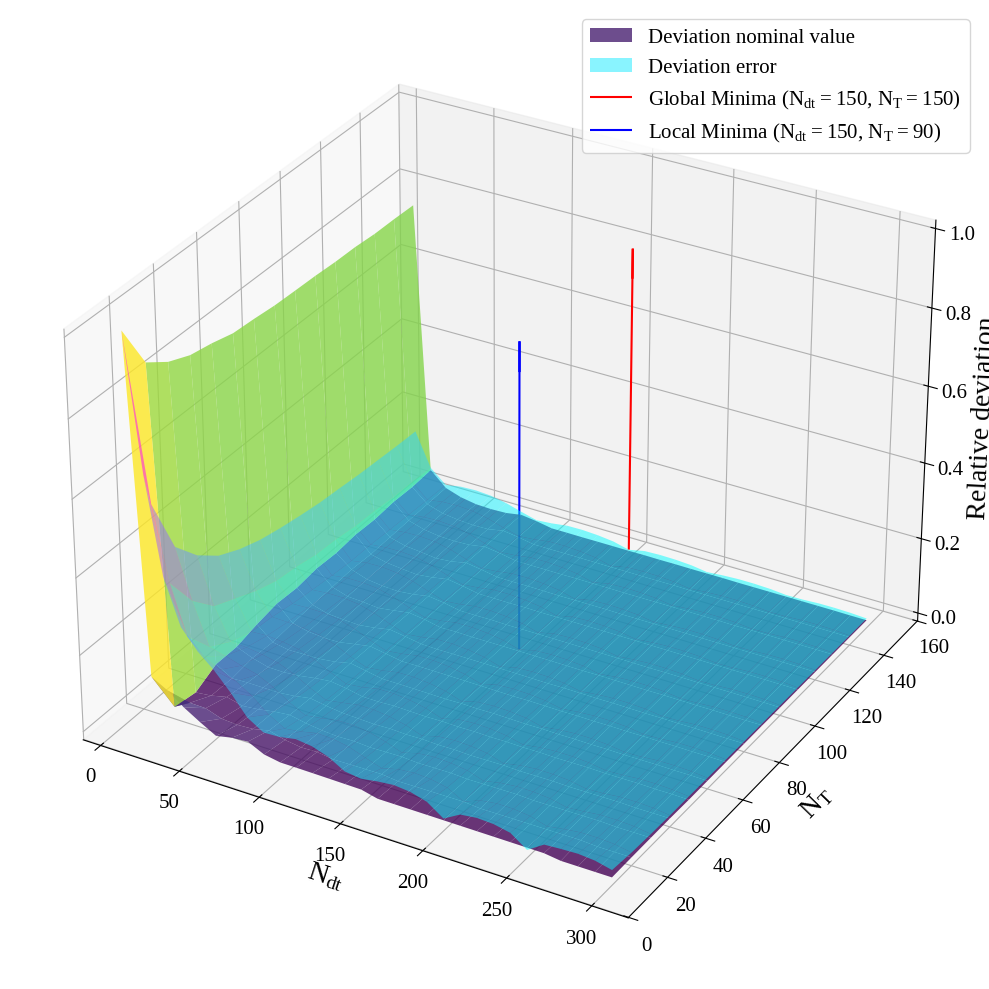
\includegraphics[width=0.5\textwidth]{3d_deviation.png}
                \caption{Závislost odchylky úhlu posunu perehelia od teoretické hodnoty na hodnotách $\text{N}_{\text{T}}$ a $\text{N}_{\text{dt}}$.}
                \label{fig:3d_deviation}
            \end{figure}

            \begin{figure}
                \centering
                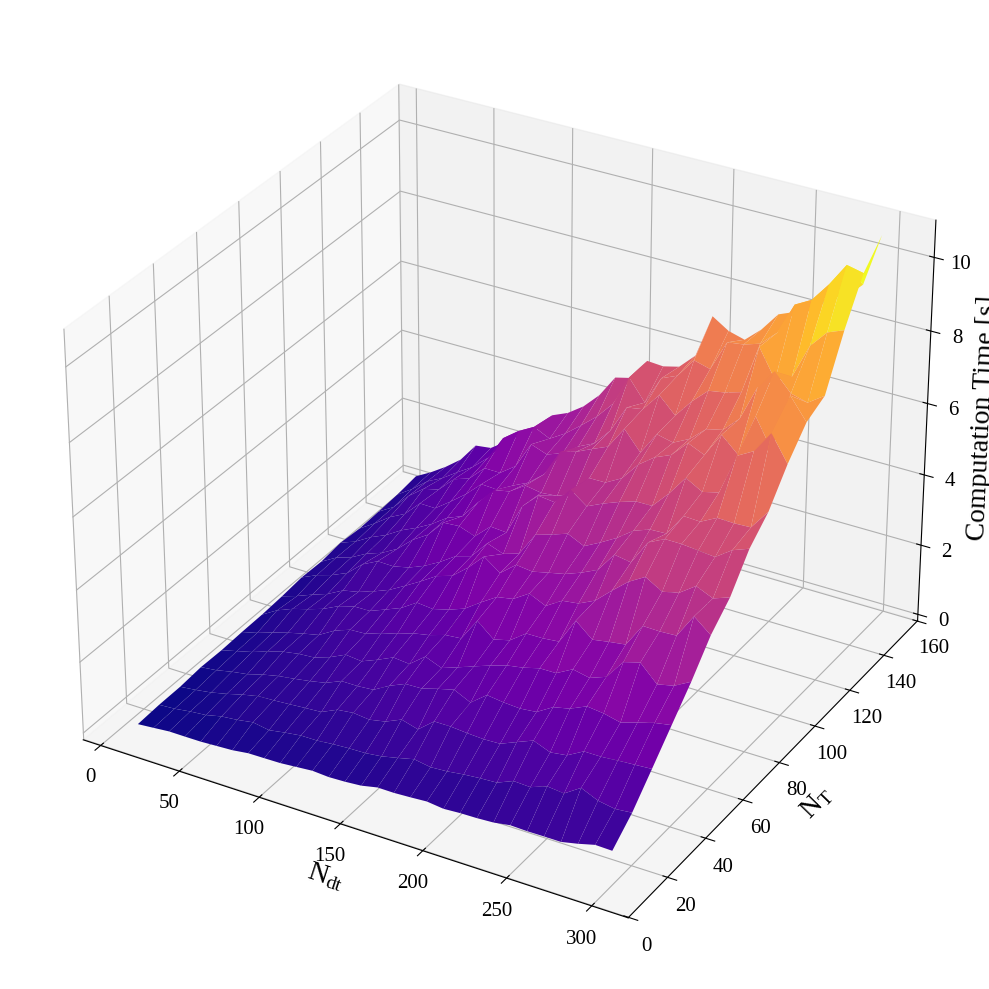
\includegraphics[width=0.5\textwidth]{3d_time.png}
                \caption{Závislost doby výpočtu na hodnotách $\text{N}_{\text{T}}$ a $\text{N}_{\text{dt}}$.}
                \label{fig:3d_time}
            \end{figure}

            Jak je vidět, s rostoucí dobou integrace a klesajícím integračním krokem se lineárně počítá doba výpočtu $t_{\text{compute}}$. Což se dalo očekávat. Pro výpočet optimálních hodnot $\text{N}_{\text{T}}$ a $\text{N}_{\text{dt}}$ budu analyzovat pouze funkce $\sigma(\text{N}_{\text{T}}, \text{N}_{\text{dt}})$ a $\sigma_{\text{err}}(\text{N}_{\text{T}}, \text{N}_{\text{dt}})$. Za tímto účelem jsem obě funkce normalizoval a sečetl do jedné funkce $\sigma_{\text{total}}(\text{N}_{\text{T}}, \text{N}_{\text{dt}})$. Poté jsem našel globální minimum této funkce (červená šipka na obrázku \ref{fig:3d_deviation}). Ukázalo se, že je to hodnota:
            
            \begin{equation*}
                \text{N}_{\text{T}} = 150, \text{N}_{\text{dt}} = 150
            \end{equation*}

            Provedením simulace s těmito hodnotami byla získána hodnota $\varphi = 43.1(3) ~[\text{arcsec/století}]$ která se liší od teoretické hodnoty o $0.2(8)\%$

            Jsem se rozhodl najít lokální minimum v oblasti hodnot $\text{N}_{\text{T}} < 100$ a $\text{N}_{\text{dt}} < 200$ (modra šipka na obrázku \ref{fig:3d_deviation}). Ukázalo se, že tato hodnota je rovna:

            \begin{equation*}
                \text{N}_{\text{T}} = 90, \text{N}_{\text{dt}} = 150
            \end{equation*}

            Provedením simulací s těmito hodnotami jsem získal hodnotu $\varphi = 43.4(5) ~[\text{arcsec/století}]$, která se od teoretické hodnoty liší o $(0.9 \pm 1.3)\%$. 
            
            Je tedy vidět, že hodnoty $\text{N}_{\text{T}}$ a $\text{N}_{\text{\text{dt}}}$ nalezené v globálním minimu jsou tedy pro tento problém optimální.

    \section{Závěr}
        Výsledky simulace ukazují uspokojivé výsledky, které se shodují s teoretickými údaji z literatury $\varphi = 43.1(3) ~[\text{arcsec/století}]$. Pro tento problém jsme také našli optimální hodnoty parametrů $\alpha$ a $\beta$: $\alpha = 0$, $\beta = 1.1 \times 10^5$. Také jsme našli optimální hodnoty $\text{N}_{\text{T}}$ a $\text{N}_{\text{dt}}$: $\text{N}_{\text{dt}}$: $\text{N}_{\text{T}} = 150$, $\text{N}_{\text{dt}} = 150$. To vše nás vede k závěru, že tento model je pro danou úlohu vyhovující. 
        
        Mezi věci, které lze zlepšit, patří doba výpočtu. Při hledání optimálních parametrů v části \ref{sec:optimal} bylo globální minimum nalezeno v suboptimálních mezích z hlediska výpočetního času. Zároveň se ukázalo, že hodnoty na výstupu jsou poměrně přesné. Možná, že změna některých kroků v procesu integrace by mohla proces optimalizovat lepším způsobem. 

    % \newpage
    \bibliographystyle{abbrvnat}
    \bibliography{bibliography}

    \section*{Poděkování}
        Tato práce byla inspirována článkem \citet{korber2018}. Jedná se o skvělou práci, a to jak z pedagogického, tak praktického hlediska. Převzal jsem z něj to nejlepší a některé tipy použil ve své analýze. 

\end{document}